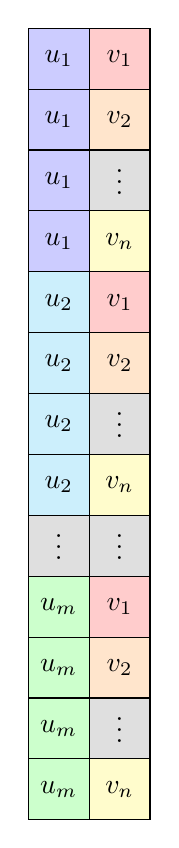
\begin{tikzpicture}
  \tikzset{square node/.style={draw, minimum size=2.2em}}

    \definecolor{verylightgray}{rgb}{0.9, 0.9, 0.9}
    \colorlet{color1}{blue!20}
    \colorlet{color2}{cyan!20}
    \colorlet{color3}{green!20}

    \colorlet{colorA}{red!20}
    \colorlet{colorB}{orange!20}
    \colorlet{colorC}{yellow!20}

  \def\x{2.2em}

    % 1
    \node[square node, fill=color1] at (\x,-\x) {$u_1$};
    \node[square node, fill=colorA] at (2*\x,-\x) {$v_1$};

    \node[square node, fill=color1] at (\x,-2*\x) {$u_1$};
    \node[square node, fill=colorB] at (2*\x,-2*\x) {$v_2$};
    
    \node[square node, fill=color1] at (\x,-3*\x) {$u_1$};
    \node[square node, fill=lightgray!50] (d1) at (2*\x,-3*\x) {};
    \node[draw=none] at (d1) [yshift=0.25em] {$\vdots$};

    \node[square node, fill=color1] at (\x,-4*\x) {$u_1$};
    \node[square node, fill=colorC] at (2*\x,-4*\x) {$v_n$};

     % 2
    \node[square node, fill=color2] at (\x,-5*\x) {$u_2$};
    \node[square node, fill=colorA] at (2*\x,-5*\x) {$v_1$};

    \node[square node, fill=color2] at (\x,-6*\x) {$u_2$};
    \node[square node, fill=colorB] at (2*\x,-6*\x) {$v_2$};
    
    \node[square node, fill=color2] at (\x,-7*\x) {$u_2$};
    \node[square node, fill=lightgray!50] (d2) at (2*\x,-7*\x) {};
    \node[draw=none] at (d2) [yshift=0.25em] {$\vdots$};

    \node[square node, fill=color2] at (\x,-8*\x) {$u_2$};
    \node[square node, fill=colorC] at (2*\x,-8*\x) {$v_n$};

    % ...
    \node[square node, fill=lightgray!50] (d3) at (\x,-9*\x) {};
    \node[draw=none] at (d3) [yshift=0.25em] {$\vdots$};
    \node[square node, fill=lightgray!50] (d4) at (2*\x,-9*\x) {};
    \node[draw=none] at (d4) [yshift=0.25em] {$\vdots$};

    % m
    \node[square node, fill=color3] at (\x,-10*\x) {$u_m$};
    \node[square node, fill=colorA] at (2*\x,-10*\x) {$v_1$};

    \node[square node, fill=color3] at (\x,-11*\x) {$u_m$};
    \node[square node, fill=colorB] at (2*\x,-11*\x) {$v_2$};
    
    \node[square node, fill=color3] at (\x,-12*\x) {$u_m$};
    \node[square node, fill=lightgray!50] (d5) at (2*\x,-12*\x) {};
    \node[draw=none] at (d5) [yshift=0.25em] {$\vdots$};

    \node[square node, fill=color3] at (\x,-13*\x) {$u_m$};
    \node[square node, fill=colorC] at (2*\x,-13*\x) {$v_n$};

\end{tikzpicture}